\documentclass{beamer}\usepackage[]{graphicx}\usepackage[]{color}
%% maxwidth is the original width if it is less than linewidth
%% otherwise use linewidth (to make sure the graphics do not exceed the margin)
\makeatletter
\def\maxwidth{ %
  \ifdim\Gin@nat@width>\linewidth
    \linewidth
  \else
    \Gin@nat@width
  \fi
}
\makeatother

\definecolor{fgcolor}{rgb}{0.345, 0.345, 0.345}
\newcommand{\hlnum}[1]{\textcolor[rgb]{0.686,0.059,0.569}{#1}}%
\newcommand{\hlstr}[1]{\textcolor[rgb]{0.192,0.494,0.8}{#1}}%
\newcommand{\hlcom}[1]{\textcolor[rgb]{0.678,0.584,0.686}{\textit{#1}}}%
\newcommand{\hlopt}[1]{\textcolor[rgb]{0,0,0}{#1}}%
\newcommand{\hlstd}[1]{\textcolor[rgb]{0.345,0.345,0.345}{#1}}%
\newcommand{\hlkwa}[1]{\textcolor[rgb]{0.161,0.373,0.58}{\textbf{#1}}}%
\newcommand{\hlkwb}[1]{\textcolor[rgb]{0.69,0.353,0.396}{#1}}%
\newcommand{\hlkwc}[1]{\textcolor[rgb]{0.333,0.667,0.333}{#1}}%
\newcommand{\hlkwd}[1]{\textcolor[rgb]{0.737,0.353,0.396}{\textbf{#1}}}%
\let\hlipl\hlkwb

\usepackage{framed}
\makeatletter
\newenvironment{kframe}{%
 \def\at@end@of@kframe{}%
 \ifinner\ifhmode%
  \def\at@end@of@kframe{\end{minipage}}%
  \begin{minipage}{\columnwidth}%
 \fi\fi%
 \def\FrameCommand##1{\hskip\@totalleftmargin \hskip-\fboxsep
 \colorbox{shadecolor}{##1}\hskip-\fboxsep
     % There is no \\@totalrightmargin, so:
     \hskip-\linewidth \hskip-\@totalleftmargin \hskip\columnwidth}%
 \MakeFramed {\advance\hsize-\width
   \@totalleftmargin\z@ \linewidth\hsize
   \@setminipage}}%
 {\par\unskip\endMakeFramed%
 \at@end@of@kframe}
\makeatother

\definecolor{shadecolor}{rgb}{.97, .97, .97}
\definecolor{messagecolor}{rgb}{0, 0, 0}
\definecolor{warningcolor}{rgb}{1, 0, 1}
\definecolor{errorcolor}{rgb}{1, 0, 0}
\newenvironment{knitrout}{}{} % an empty environment to be redefined in TeX

\usepackage{alltt}
\usepackage{../371g-slides}
% Uncomment these lines to print notes pages
% \pgfpagesuselayout{4 on 1}[letterpaper,border shrink=5mm,landscape]
% \setbeameroption{show only notes}
\title{Introduction to predictive analytics}
\subtitle{Lecture 1}
\author{STA 371G}
\IfFileExists{upquote.sty}{\usepackage{upquote}}{}
\begin{document}



  \frame{\maketitle}

  % Show outline at beginning of each section
  \AtBeginSection[]{
    \begin{frame}<beamer>
      \tableofcontents[currentsection]
    \end{frame}
  }

  %%%%%%% Slides start here %%%%%%%

  \begin{darkframes}
    \begin{frame}{Course goals}
      \begin{itemize}
        \item Use regression and time series analysis to build predictive models
        \item Build decision trees to help make decisions under uncertainty
        \item Utilize simulations to forecast outputs based on uncertain inputs
        \item Given a new business situation, select an appropriate analysis, carry it out, and effectively communicate the results
        \item \alert{This is a practical course!}
      \end{itemize}
    \end{frame}

    % TODO: Update for instructor
    \begin{frame}{About the course staff}
      \begin{itemize}
        \item Instructor: \textbf{Brian Lukoff, Ph.D.}
          \begin{itemize}
            \item Office hours: M/W 11 AM - 12 PM in CBA 3.440
            \item Contact: \texttt{brian.lukoff@utexas.edu} or 415-652-8853
          \end{itemize}
        \item TAs:
          \begin{itemize}
            \item Office hours: W/Th/F 2-4 PM in CBA 4.304A
            \item Help session: F 11 AM - 12 PM in the ModLab
          \end{itemize}

          \vspace{0.2in}
          \begin{tabular}{ccc}
            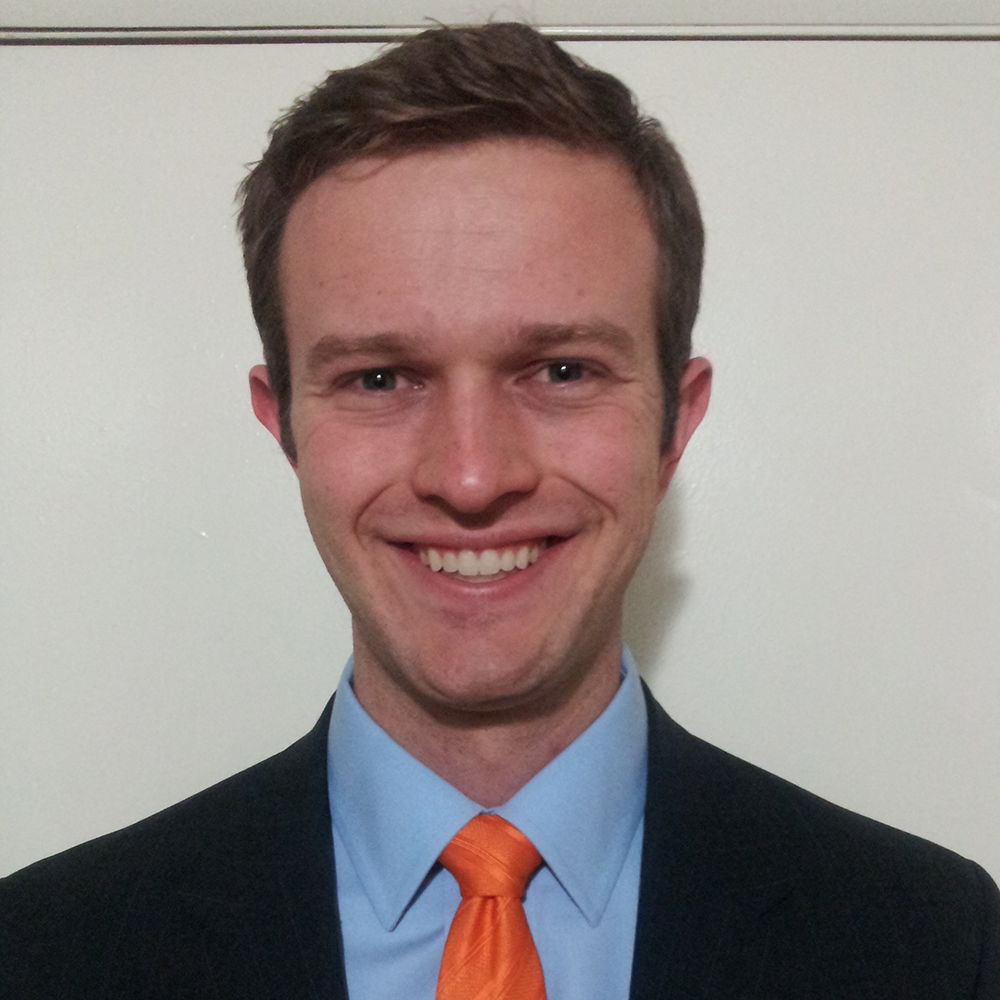
\includegraphics[width=0.8in]{jared} &
            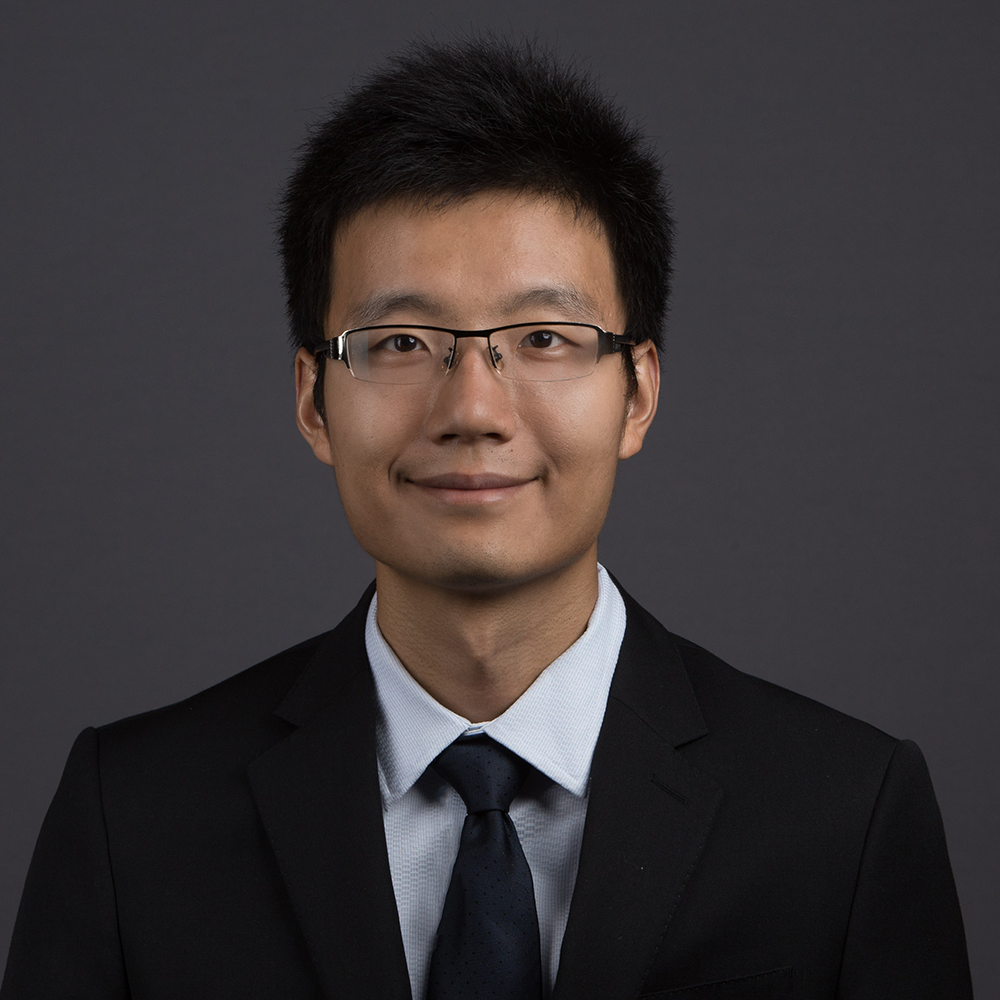
\includegraphics[width=0.8in]{han} &
            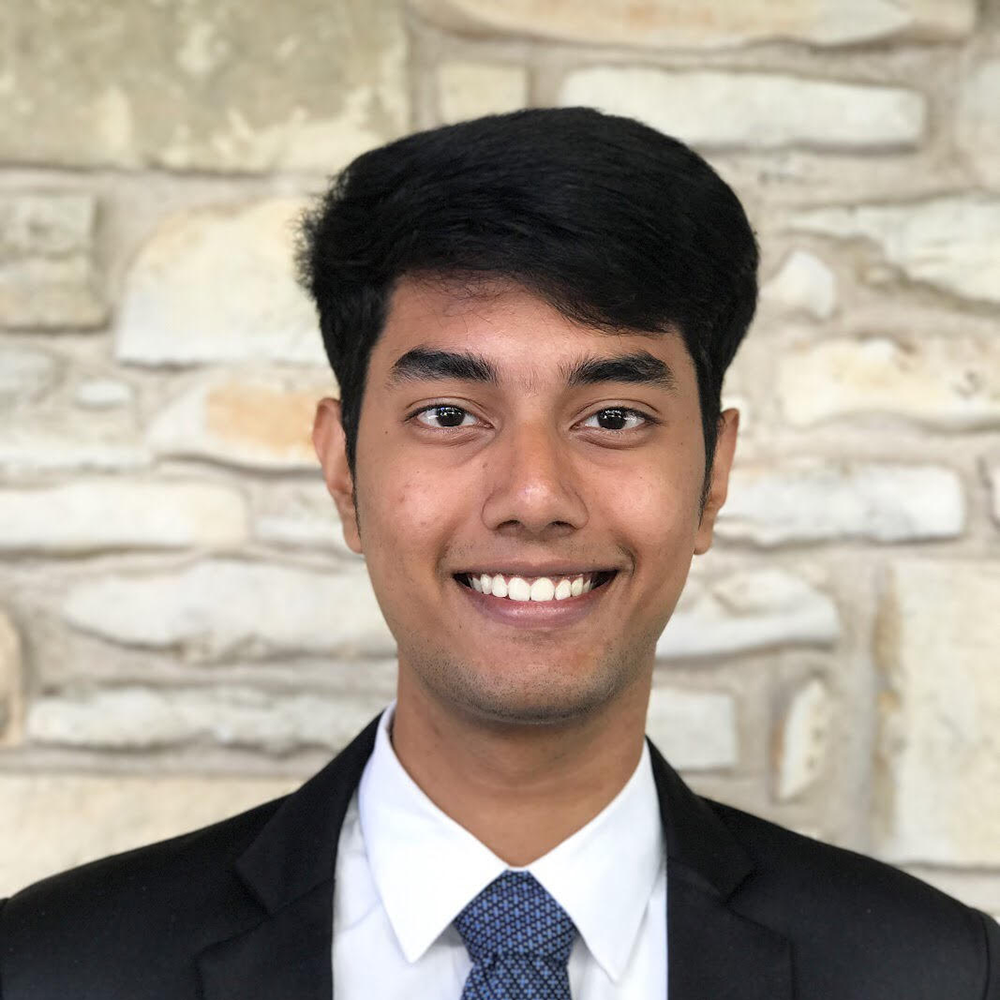
\includegraphics[width=0.8in]{sai} \\
            Jared Fisher & Han Jiang & Sai Ravi \\
          \end{tabular}
      \end{itemize}
    \end{frame}

    % TODO: Update for instructor
    \begin{frame}{Who am I?}
      \begin{itemize}
        \item \textbf{Educator:} Previously taught at Harvard University and Boston University
        \item \textbf{Entrepreneur:} Currently co-founder and CEO of Perusall; formerly co-founder and CEO of Learning Catalytics (acquired by Pearson)
        \item \textbf{Engineer/statistician:} Software engineering/analytics background
      \end{itemize}
    \end{frame}

    \section{Find someone who...}

    \begin{frame}{}
      \begin{center}
        For each box on your bingo card, find someone who matches the description in the box. You must use a different person for each box.
        \vfill
        The winner will be crowned the STA 371G Bingo Champion$^{\text{TM}}$.
      \end{center}
    \end{frame}

    \section{Course logistics}

    \begin{frame}{Canvas}
      \begin{itemize}
        \item Access at \url{canvas.utexas.edu}
        \item This is your home base for the course
        \item Make sure you can log in and are enrolled in STA 371G in Canvas
      \end{itemize}
    \end{frame}

    \begin{frame}{Class participation}
      \begin{itemize}
        \item We will use \alert{Learning Catalytics} so you can get practice of the concepts during class
        \item Buy online (\$12) at \url{learningcatalytics.com} or use for free if you bought for another class (you may still have access from STA 309)
        \item Grading based on completeness only; answer 75\% of the questions for full credit
        \item Bring a laptop, smartphone, or tablet to every class
        \item A note about devices in class
      \end{itemize}
    \end{frame}

    \begin{frame}{Reading assignments}
      \begin{itemize}
        \item No textbook is required for this course
        \item We will use \alert{Perusall} for reading assignments
        \item Access for free at \url{perusall.com}
        \item Use Perusall to ask and answer your classmates questions and have discussions in the text
        \item This will help you better understand the text and will help me gear class time to what topics you are having the most trouble with
        \item Reading assignments are due by 7 PM; grading is based on effort and thoughtfulness of your questions and comments
      \end{itemize}
    \end{frame}

    \begin{frame}{Statistical computing}
      \begin{columns}[onlytextwidth]
        \column{.6\textwidth}
          \begin{itemize}
            \item We will use \alert{R} for statistical analysis throughout the course
            \item This is industrial-strength, state-of-the-art, and free software for statistical computing
            \item We will access R through \alert{RStudio}, a graphical interface for R
            \item Download R and RStudio at \url{rstudio.com}
          \end{itemize}
        \column{.3\textwidth}
          
\includegraphics[width=1in]{R}
      \end{columns}
    \end{frame}

    \begin{frame}{Homework}
      \note{Make the point that we don't give busywork in 371. \textCR
      We only give them work that will help them learn.}
      \begin{itemize}
        \item Regular homework assignments during the semester
        \item Submit in QUEST by 11:59 PM on the due date
        \item Why homework?
      \end{itemize}
    \end{frame}

    \begin{frame}{Exams}
      \begin{itemize}
        \item Two midterm exams and a cumulative final exam
        \item All are given outside of class times; you'll sign up for a time that is convenient for you
        \item Tests are in the ModLab; you'll have access to R during every exam
        \item Your final exam will overwrite your lowest midterm grade if it helps your overall grade
      \end{itemize}
    \end{frame}

    \begin{frame}{Team project}
      \begin{itemize}
        \item One team project
        \item You will pick a data set (or create one, e.g. through a survey) and apply regression techniques (we'll learn about this!) to build a predictive model
      \end{itemize}
    \end{frame}

    \begin{frame}{Grading}
      \begin{center}
        \begin{tabular}{ll}
          Class participation & \textbf{5\%}  \\
          Reading assignments & \textbf{5\%}  \\
          Homework   & \textbf{15\%} \\
          Team project & \textbf{15\%} \\
          Midterm 1  & \textbf{20\%} \\
          Midterm 2  & \textbf{20\%} \\
          Final Exam & \textbf{20\%} \\
        \end{tabular}
      \end{center}
    \end{frame}

    \section{Let's do some statistics, yo}

    \begin{frame}{Purpose of a model}
      \begin{itemize}
        \item \textbf{Make a prediction} about one variable based on the others
        \item \textbf{Understand the relationships} between the variables
      \end{itemize}
    \end{frame}

    \begin{frame}{Data analysis process}
      \begin{center}
        \tikzstyle{block} = [rectangle, draw, fill=darkgray,
            text width=8em, text centered, rounded corners, minimum height=2em]
        \tikzstyle{line} = [draw, -latex']

        \begin{tikzpicture}[node distance = 1.4cm, auto]
          \node [block] (define) {define problem};
          \node [block, below of=define] (explore) {explore the data};
          \node [block, below of=explore] (build) {build model};
          \node [block, below of=build] (evaluate) {evaluate model};
          \node [block, below of=evaluate] (conclude) {make conclusions};
          \path [line] (define) -- (explore);
          \path [line] (explore) -- (build);
          \path [line] (build) -- (evaluate);
          \path [line] (evaluate) -- (conclude);
        \end{tikzpicture}
      \end{center}
    \end{frame}

    \begin{frame}{Define the problem}
      \note{Ask the class to brainstorm. \textCR
      The first answer will probably be "how well the instructor teaches", \textCR
      but ask them what other characteristics might affect ratings, even \textCR
      subconsciously.}
      \begin{center}
        What personal characteristics about an instructor do you think are predictive of the scores they receive on student evaluations?
      \end{center}
    \end{frame}

    \begin{frame}
      \note{Emphasize that this is real data, and from UT to boot.}
      
\includegraphics[width=\textwidth]{hamermesh}
    \end{frame}

    \begin{frame}{Hamermesh \& Parker (2004) data set}
      \begin{itemize}
        \item Student evaluations of $N=463$ instructors at UT Austin, 2000-2002
        \item For each instructor:
          \begin{itemize}
            \item \textbf{beauty}: average score from a six-student panel)
            \item \textbf{gender}: male or female
            \item \textbf{credits}: single- or multi-credit course
            \item \textbf{age}: age of instructor
            \item (and more...)
          \end{itemize}
      \end{itemize}
    \end{frame}

    

    \begin{frame}{Explore the data}
      \note{
        Before showing this, ask students how you might explore the impact \textCR
        of gender on evaluation scores. If someone suggests comparing the \textCR
        means, ask how you might graphically display it. \textCR
        After displaying the graph, elicit what we can conclude---the mean \textCR
        is higher for men, but the spread also looks larger.  Use this as \textCR
        an opportunity to quickly review variance/SD.
      }
\begin{knitrout}
\definecolor{shadecolor}{rgb}{0.969, 0.969, 0.969}
\input{/tmp/figures/unnamed-chunk-3-1.tikz}

\end{knitrout}
    \end{frame}

    \begin{frame}{Explore the data}
      \note{
        Before showing this, ask students how you might explore the impact of \textCR
        single vs multi credit courses on evaluation scores. Ask students to \textCR
        speculate on the cause.
      }
\begin{knitrout}
\definecolor{shadecolor}{rgb}{0.969, 0.969, 0.969}
\input{/tmp/figures/unnamed-chunk-4-1.tikz}

\end{knitrout}
    \end{frame}

    \begin{frame}{Explore the data}
      \note{
        Before showing this, ask students how you might explore the impact of \textCR
        beauty on evaluation scores, and ask students to predict the effect.
      }
\begin{knitrout}
\definecolor{shadecolor}{rgb}{0.969, 0.969, 0.969}
\input{/tmp/figures/unnamed-chunk-5-1.tikz}

\end{knitrout}
    \end{frame}

    \begin{frame}{Explore the data}
      \note{
        Before showing this, ask students to predict the effect of age on \textCR
        evaluation scores.
      }
\begin{knitrout}
\definecolor{shadecolor}{rgb}{0.969, 0.969, 0.969}
\input{/tmp/figures/unnamed-chunk-6-1.tikz}

\end{knitrout}
    \end{frame}

    \begin{frame}{Build the model}
      
      \begin{center}
        A regression model lets us create a model that incorporates all of these relationships to best predict evaluation scores:
        \[
          \widehat{\text{eval}} =
            4.13 +
            0.16 \cdot \text{beauty} -
            0.2 \cdot \text{female} +
            0.58 \cdot \text{credits} +
            0 \cdot \text{age}
        \]

        \pause

        We predict a 40-year-old female, with a beauty score of 2, teaching a multi-credit course would get an evaluation score of
        \[
          \widehat{\text{eval}} = 4.13 + 0.16 \cdot 2 - 0.2 \cdot 1 + 0.58 \cdot 0 = 4.18.
        \]

      \end{center}
    \end{frame}

    \begin{frame}{Evaluate the model}
      How could you evaluate the quality of this model?
    \end{frame}

    \begin{frame}{Can we do better?}
      \note{
        The pattern is different for men and women---beauty makes more of \textCR
        a difference for men. We probably will not have time to go into it\textCR
        any further; this is just to whet students' appetite for what is possible.
      }
      Do you see a different pattern between men and women?

\begin{knitrout}
\definecolor{shadecolor}{rgb}{0.969, 0.969, 0.969}
\input{/tmp/figures/unnamed-chunk-8-1.tikz}

\end{knitrout}
    \end{frame}

    \begin{frame}{Six for the weekend}
      \begin{enumerate}
        \item Read the syllabus
        \item Install R and RStudio on your computer
        \item Make sure you can log in to Canvas
        \item Purchase (or see if you already have access to) Learning Catalytics
        \item Create a Perusall account
        \item Bring a device to class on Monday
      \end{enumerate}
    \end{frame}


  \end{darkframes}

\end{document}
